\chapter{Objetivos y metodología}\label{chap:objetivos}

Se procede a explicar en este capítulo los objetivos concretos y la metodología de trabajo que van a marcar cómo se materializará la contribución que se va a realizar.

\section{Objetivo general}\label{sec:objgeneral}
El objetivo general del presente trabajo es extender la capacidad de monitorización que se tiene sobre una red empresarial.
Se enfocará para ello en la detección de anomalías, haciendo uso de técnicas basadas en los equipos que la componen (a diferencia de las basadas en flujos de tráfico).
De este modo, se desarrollará un sistema que categorice mediante \emph{clustering} los equipos informáticos finales (es decir, todos menos la infraestructura de la red)
y que pueda revelar cuándo la actividad de un equipo se desvía de su comportamiento habitual.

Con ello se espera seguir mejorando las prestaciones ofrecidas, especialmente en seguridad, pero también ayudará en la identificación de problemas de configuración, cambios de tendencia en la red y en definitiva cualquier evento inesperado que pudiera repercutir negativamente en la operativa normal de la empresa monitorizada.

\section{Objetivos específicos}\label{sec:objespecificos}
La consecución de dicho objetivo general vendrá pautada por las siguientes metas más específicas, que se abordarán en este orden:

\begin{itemize}

\item Determinar qué características son las más relevantes a la hora de \emph{clusterizar} la red y extraerlas en tiempo real.

\item Establecer unas categorías básicas mediante clasificación no supervisada, que sean verificables con la documentación que se tiene de la red.

\item Comprobar que el sistema detecta anomalías.

\item Refinar el algoritmo de \emph{clustering} empleado, buscando categorías más específicas que no se estuvieran teniendo en cuenta antes.

\item Alcanzar un modo de funcionamiento en tiempo real, en coordinación con los demás mecanismos de monitorización presentes y asegurando una precisión razonable.

\end{itemize}

\section{Metodología de trabajo}\label{sec:metodologiatrabajo}

Con los anteriores objetivos específicos marcados, se hace necesario establecer un marco de trabajo para llevarlos a cabo.
En esta sección se estructurará una metodología de trabajo en base a cuatro fases, que tienen como fin último alcanzar el objetivo general.
Sus enunciados vendrán acompañados de una descripción, explicando con un poco más de detalle cómo se planea ejecutar cada etapa.

\begin{itemize}

    \item Selección de las características más relevantes para la clasificación

A partir de la heterogénea colección de logs de varios firewalls de la que se dispone, se identificarán los datos que puedan ser interesantes para el \emph{clustering}.
Se tendrán en cuenta distintos aspectos que respondan a las actividades que realiza un equipo informático en una red empresarial, como por ejemplo la cantidad de conexiones, sus duraciones, horarios de actividad, interacción con ciertos servidores, etc.
A continuación, se analizarán estas características a través de técnicas estadísticas, gracias a las cuales se adquirirá un entendimiento preliminar de la importancia que cada una supone para la posterior clasificación de instancias.
Es posible que se logre la reducción de su dimensionalidad, la eliminación de alguna característica redundante o en definitiva alguna simplificación que haga el \emph{clustering} más sencillo de ejecutar.

    \item Obtención de categorías mediante \emph{clustering}

Se pasará entonces a aplicar por primera vez algunos métodos de \emph{clustering} sobre estos datos.
Lo que se pretende es categorizar los equipos en su comportamiento ``normal'', de forma que se tengan clasificados en varios tipos según su actividad.
Inicialmente se elegirá un algoritmo simple y ampliamente conocido como es K-Means, con variaciones sobre él.
Se experimentará con diferentes valores para sus parámetros, ya que así podrán compararse resultados.
De cara a determinar la efectividad de los algoritmos, se considerarán medidas objetivas que representen su rendimiento.
Los métodos típicos para ello valoran características intrínsecas o derivadas como su complejidad, estabilidad y tiempo de computación, así como la suma de cuadrados de las desviaciones.
Además, se emplearán los indicadores comunes con los que se suele definir la bondad de una técnica de clasificación en aprendizaje automático.

    \item Detección de anomalías con análisis del \emph{clustering}

Una vez se cuente con una clasificación satisfactoria, se procederá a la siguiente fase, en la cual se aspira a detectar anomalías en los datos.
En caso de contar con instancias que se hayan identificado como anomalías mediante otros métodos, se usarán para probar la capacidad de detección del sistema.
Dado que también se desea detectar otras clases de anomalías más genéricas (no solo relacionadas con seguridad), se incluirán casos como cambios de configuración o de equipos que hayan cambiado de rol en la red.

    \item Evaluación en escenario real

Finalmente, se desplegará el sistema desarrollado en un entorno de producción.
Se ofrecerá una representación visual adecuada que permita al analista aprovechar el valor que el sistema aportará a la hora de revisar casos alertados.
Además, se automatizará la extracción de características y se prepararán el resto de componentes del sistema para que funcione lo más cercano a tiempo real posible.

\end{itemize}

\section{Metodología del desarrollo}\label{sec:metodologiadesarrollo}

Tras haber completado las fases del desarrollo requeridas para poner en funcionamiento este piloto y haber analizado y probado lo que mejor funcionaba en cada una,
se ha plasmado la metodología seguida en esta serie de pasos, que ofrecen una visión global del desarrollo que se ampliará en el capítulo \ref{chap:desarrollo}:

\begin{itemize}

\item A partir de logs en bruto de firewall, extracción de los vectores de características de las sesiones.

\item Preprocesado antes del \emph{clustering}:

    \begin{itemize}

        \item Muestreo (necesario para el desarrollo, pero prescindible cuando se lleve a producción).

        \item Transformación de los datos individuales en características para la entrada del \emph{clustering},
            formada básicamente, por un lado, por la agrupación diaria y por IP origen, y por otro, por el cálculo de las métricas con las que se ha decidido trabajar.

        \item Normalización de estos datos.

    \end{itemize}

\item Aplicación de KMeans con $k=5$

\item Análisis:

    \begin{itemize}

        \item Revisión manual en el entorno de la empresa de las IP clasificadas como anomalías.

        \item Evaluación de la estabilidad del resto de \emph{clusters} normales, para vigilar si hay cambios de tendencia.

    \end{itemize}

\end{itemize}

El siguiente esquema de la figura \ref{fig:esquema} resume todo el procesado:

\begin{figure}[h]
    \centering
    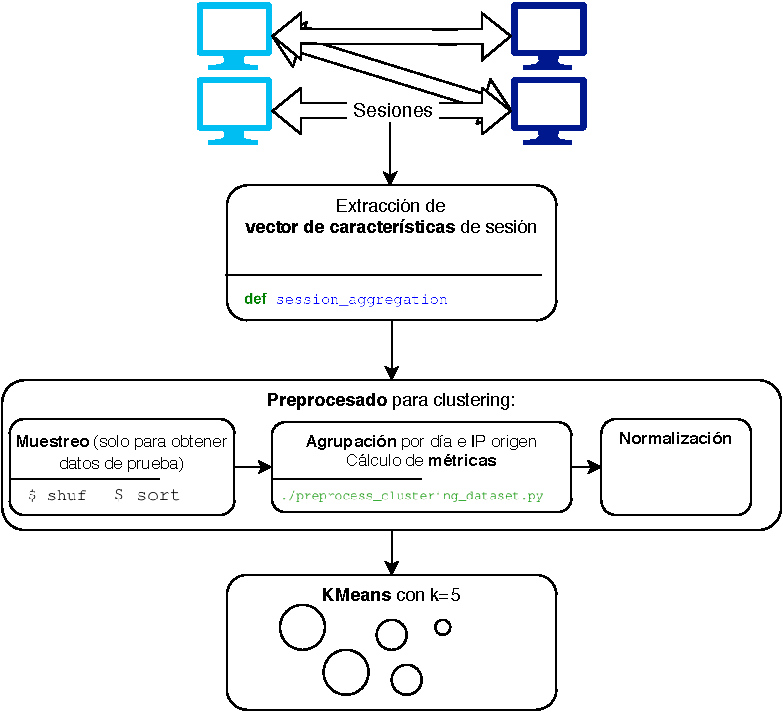
\includegraphics{contenido/fig/esquema.pdf}
    \caption{Diagrama de la metodología seguida en el procesado}
    \label{fig:esquema}
\end{figure}
